\documentclass[12pt,letterpaper,noanswers]{exam}
\usepackage[usenames,dvipsnames,svgnames,table]{xcolor}
\usepackage[margin=0.9in]{geometry}
\renewcommand{\familydefault}{\sfdefault}
\usepackage{multicol}
\pagestyle{head}
\header{AM 108 Class 26}{}{Maps}
\runningheadrule
\headrule
\usepackage{graphicx} % more modern
\usepackage{amsmath} 
\usepackage{amssymb} 
\usepackage{hyperref}
\usepackage{tcolorbox}

\begin{document}
 \pdfpageheight 11in 
  \pdfpagewidth 8.5in

\noindent 




\begin{itemize}
\itemsep0em
\item You'll receive feedback on your proposals by the end of today.  You have a log due Friday.
\item There is a 2d system analysis due Friday Nov 13th (to be done independently - you will have access to us in office hours, but we will meet with you individually in a breakout room).
\item There is a pre-class assignment for Wednesday.
\item There is not a new skill check for Wednesday, but there is a C24 retake.
\item I owe you a Quiz 02 Follow Up assignment.  Once I post it, the assignment deadline will be flexible.
\end{itemize}

\hrule
\vspace{0.2cm}



\noindent\textbf{Teams}

Team 1: Isaac, Emily, Annabelle

Team 2: Coco, Jaleel, Zhe

Team 3: Isaac A, Zhao, Martin, Ethan

Team 4: Daniel, Winnie, Hal

Team 5: Charlie, Dabao, Jessica

Team 6: Justin, Mark, Laura


\noindent \textbf{Teams 1 and 2}: Post screenshots of your work to the course Google Drive today.  Include words, labels, and other short notes that might make those solutions useful to you or your classmates.  Find the link in Canvas (or here: \url{https://drive.google.com/drive/u/0/folders/1GcpwvKHD4tMecpFQ4lNxN_r5Ylj7YHbd})


\vspace{0.2cm}

\hrule
\vspace{0.2cm}


\noindent\textbf{Big picture}

The logistic map is an important example.  We will study it (and other maps) to learn about one route to chaos and about the structure of an attractor.




\vspace{0.2cm}
\hrule
\vspace{0.2cm}


\noindent \textbf{Extra vocabulary / extra facts:}
\begin{tcolorbox}

A \textbf{period-doubling cascade} is a sequence of period-doubling bifurcations that appears to be an infinite sequence.  \emph{Note: these cascades have been observed experimentally (in laser systems, in circuits, in oscillating chemical reactions).}.  

The period-doubling cascade is often referred to as a \textbf{route to chaos} because they occur in deterministic systems and at the limit of the process we see aperiodic orbits with sensitive dependence on initial conditions.

For most maps, the ratio of the parameter distance between two successive period-doublings in the cascade approaches a constant of $\delta = 4.6692...$.  This is a fundamental constant (like $\pi$, but more obscure) and is known as \textbf{Feigenbaum's constant}.  

\textbf{Renormalization theory} is a method that we will use (not today) to show that the same type of period-doubling cascade as we see in the logistic map will appear in a wide range of unimodal (one-humped) maps.
\end{tcolorbox}


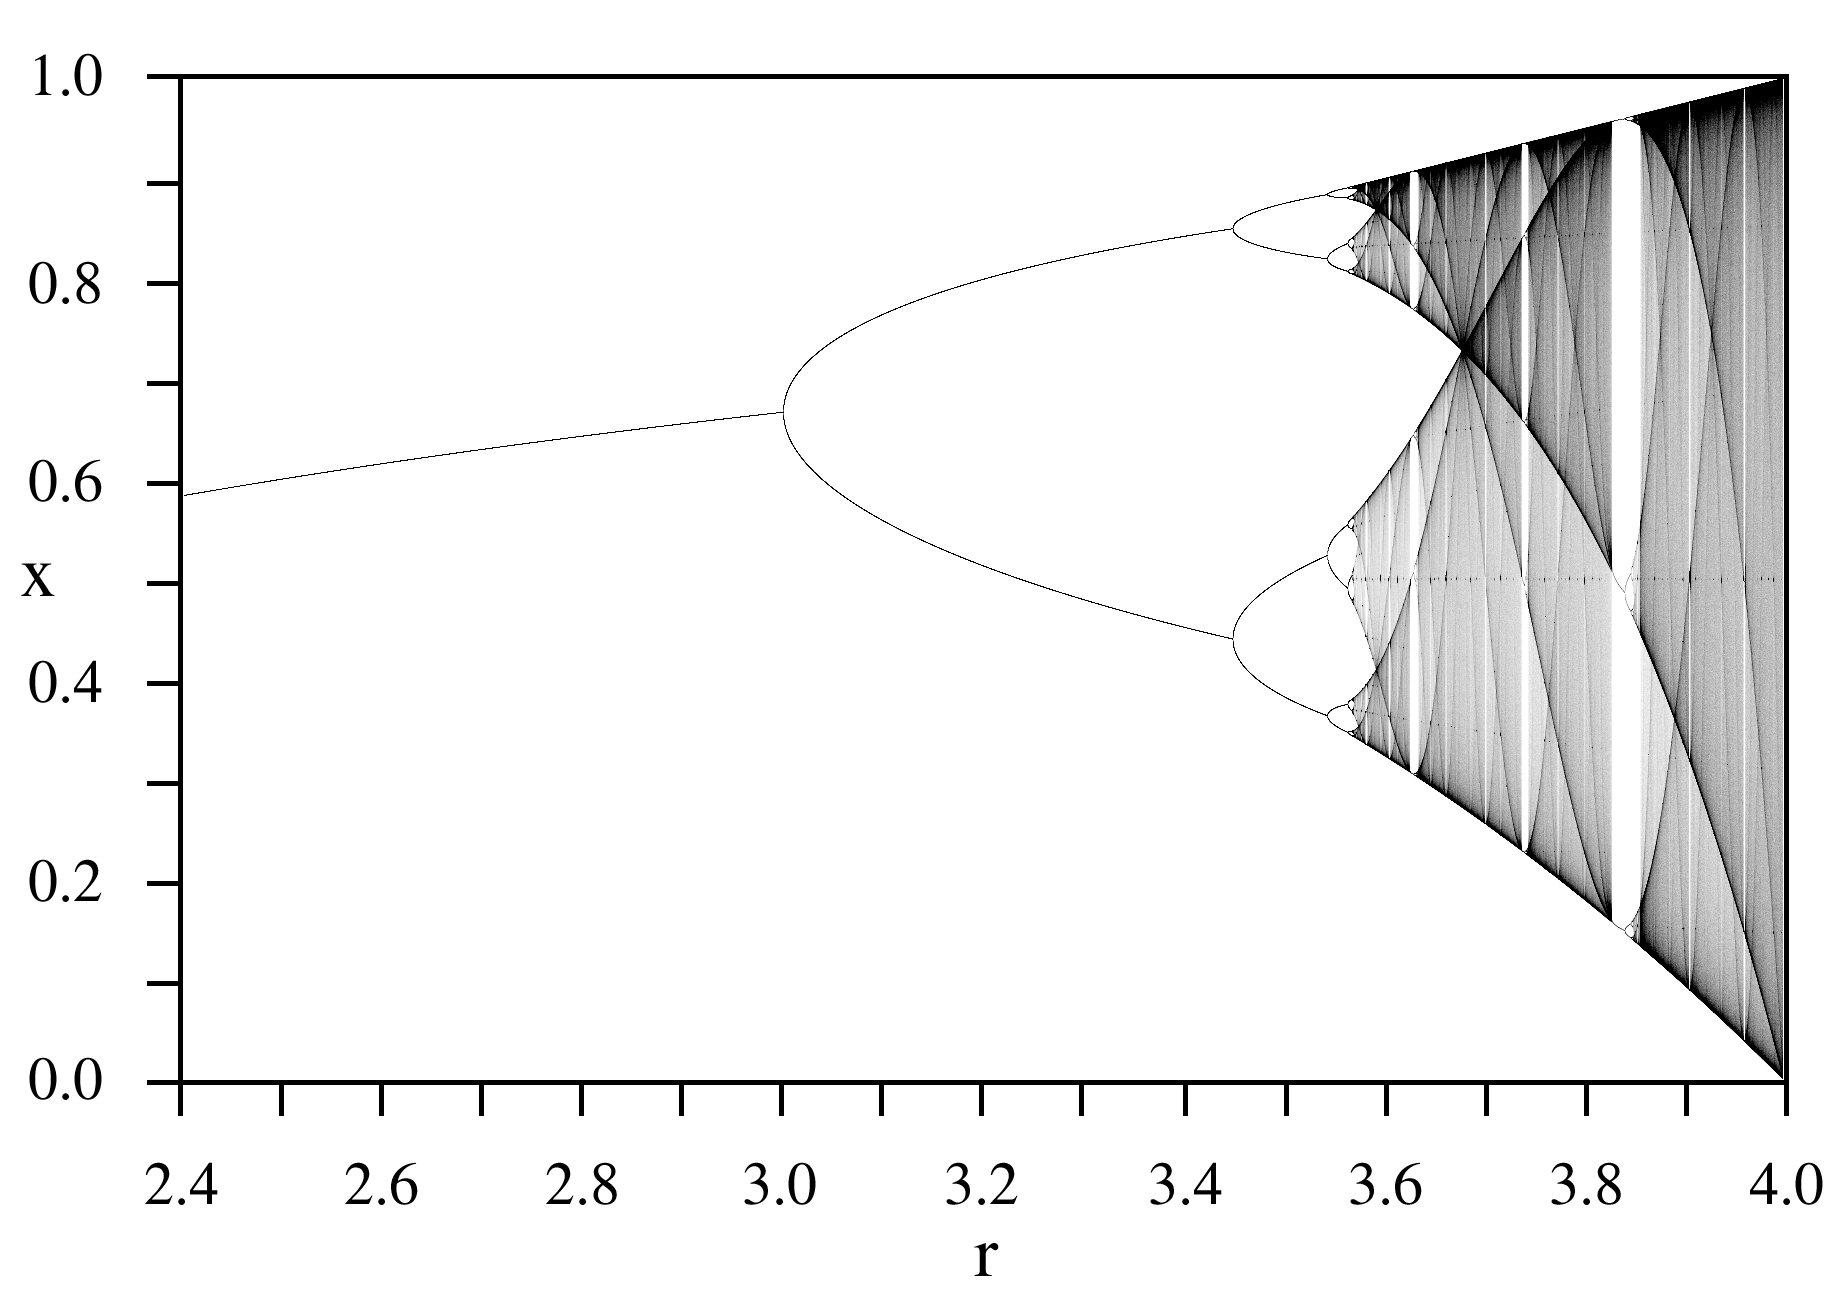
\includegraphics[width=6in]{img/logistic.png}

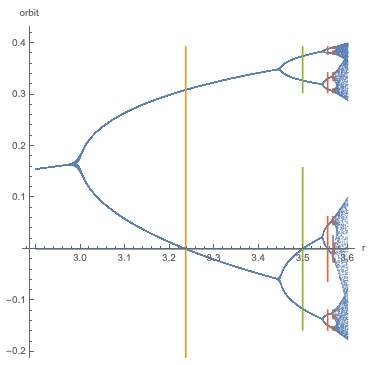
\includegraphics[width=0.45\textwidth]{img/191111-C28p1a.png}
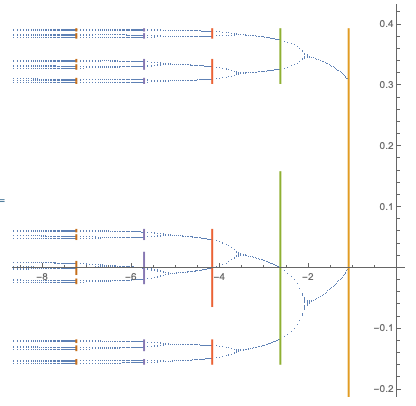
\includegraphics[width=0.45\textwidth]{img/191111-C28p1b.png}



\begin{tcolorbox}
A \textbf{shift map} is a common type of example map in which we can identify aperiodic and periodic orbits.  It is a map where you have a sequence of symbols specifying your state, $S_0S_1S_2...$ and the map shifts them over and drops the first one, so $f(S_0S_1S_2...)=S_1S_2S_3...$.  For example, for the \textbf{decimal shift map}, $f(.13257) = .3257$ 

\end{tcolorbox}

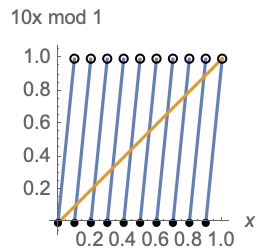
\includegraphics[scale=0.8]{img/C26shift10p1.png}
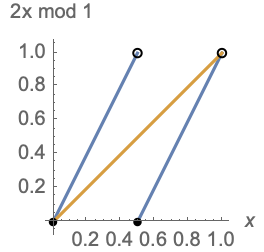
\includegraphics[scale=0.8]{img/C26shift2p2.png}

\vspace{0.2cm}
\hrule
\vspace{0.2cm}

\noindent\textbf{Skill Check C27 practice}
\begin{questions}
\item Retake of skill check C24: identify the attractor given part of a phase portrait

\item No new skill for C27.

\end{questions}

\vspace{0.2cm}

\hrule
\vspace{0.2cm}


\noindent\textbf{Questions}

\noindent \ \ 0.  Introduce yourself to your new team, and write your names on the slide.

\begin{questions}


\question (Explicit aperiodic and periodic orbits) Take a look at the decimal shift map.
\begin{parts}
\item How many fixed points does it have?  Identify them. and find their stability.
\item Give an example of a decimal sequence that would be part of a period-2 orbit.
\item Construct an example (or give an example) of a decimal sequence where the orbit will be aperiodic.
\item This type of map is sometimes said to be a `stretching and tearing' map for the interval $[0,1]$ while the logistic map (for sufficiently large $r$) is said to be a `stretching and folding' map for $[0,1]$.  Think a little bit about what people might be referring to when they call those maps `stretching'.
\end{parts}

\question 
(Example 4.9, Alligood et al) Consider the tent map $x_{n+1} = T_3(x_n),$ defined as \[
x_{n+1} = \left\{
        \begin{array}{ll}
            3x_n, & \quad 0\leq x_n \leq \frac{1}{2} \\
            3(1-x_n), & \quad \frac{1}{2}\leq x_n \leq 1.
        \end{array}
    \right.
    \]
    
For the slope-3 tent map, let $C$ be the set of points in the interval $[0,1]$ whose orbits stay in the interval $[0,1]$.  This is the set of initial conditions
that will never leave the interval under iteration of $T_3$.  The set $C$ has an interesting (fractal) structure.
\begin{parts}
\part Sketch the map.  
\part \begin{itemize}
    \item Identify the fixed points of the map.
    \item Identify points that map to zero, so $T_3(x) = 0$.
    \item Identify points whose second iterate, $T_3^2(x)$, is zero (these are points that map to points that map to zero).  
\end{itemize}   
These are all points that are part of $C$.

\part Convince your team that initial conditions in the interval $(1/3, 2/3)$ are the only points that leave the interval $[0,1]$ under a single iteration of $T_3$ (note that $1/3$ and $2/3$ both stay in the interval).  Sketch the line segments that are still in consideration for potentially being in $C$.  Call this set $C_1$.  
\part What points will leave the interval under two iterations of $T_3$?  Again sketch the line segments that are still in consideration for staying in the interval. Call this set $C_2$. Is the set of points closed or open?  (i.e. do the intervals contain their endpoints or not?)
\part Can you generalize this to sketch $C_3$ (three iterations)?  What do you think will happen with $k$ iterations?
\part What points seem to be in $C$?
\end{parts}

\item (BZ-reaction) Remember the periodic chemical reactions we saw when we learned about limit cycles?  (The beaker that turned blue, then yellow then clear, or the spatially extended BZ-reaction with its blue and red circles, spirals, and waves).

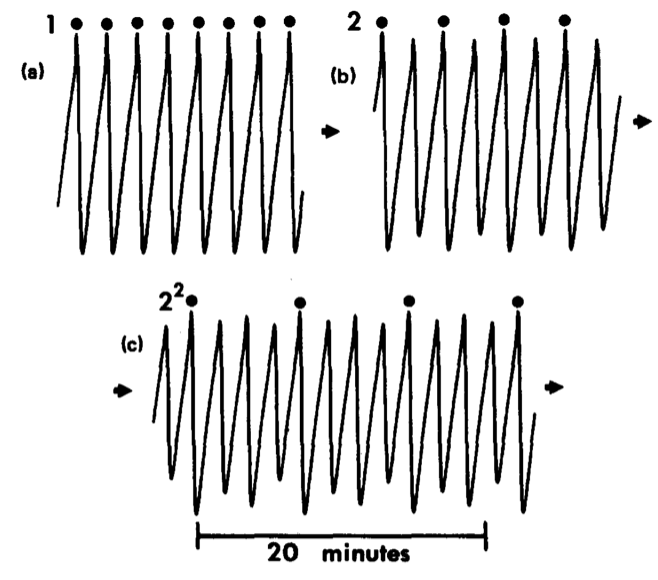
\includegraphics[width=0.55\textwidth]{img/191108-C27p3b.png}


The time-series above are showing an ion concentration from experimental measurements of bromide concentration in the BZ-reaction.  $\tau$ is the flow rate into the continuously stirred tank reactor (CSTR).

In (a), we have $\tau = 0.725$ hours.  In (b) we have $\tau = 0.773$ hours.  In (c) we have $\tau = 0.803$ hours.

\begin{parts}
\item What are the periods in (a), (b), (c)?
\item What kind of bifurcation likely happens between (a) and (b) and between (b) and (c)?
\end{parts}

\question (The Rossler system.)

The Rossler equations are:
\begin{align*}
\dot x &= -y-z \\
\dot y &= x + a y \\
\dot z &= b + z(x-c)
\end{align*}

This is a slightly simpler system then the Lorenz system (and its dissipation / volume contraction is slower).


$a = 0.2, b=0.2,c=5$ is a parameter set associated with chaos.

\begin{parts}
\item Find the nonlinear term(s) in the system.  How many are there?
\item We map a `Lorenz map' for this system using local maximum values of $x(t)$ (it looks nicer than local maxima of $z(t)$).  I'll call it the `Rossler map'.  

On the left is a trajectory with those local maxima plotted on it as tiny red dots. On the right is the resulting map (for $c = 4.5$ in red and $c=5$ in blue).

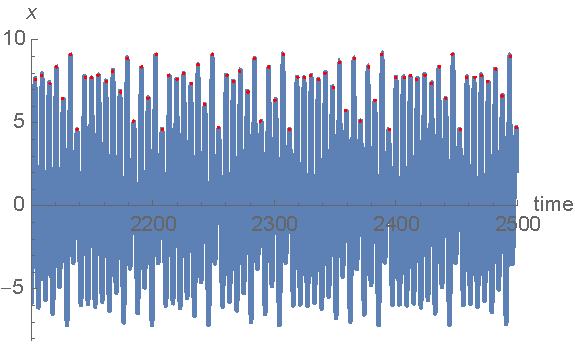
\includegraphics[scale=0.8]{img/191108-C27p5d.pdf}
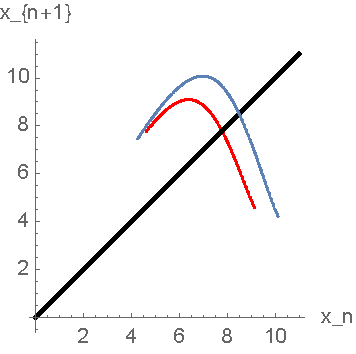
\includegraphics[scale=0.8]{img/191108-C27p5c.pdf}

Using a range of $c$ values and plotting those success maxima (so the orbit of the `Rossler map'), I have the following orbit diagram:

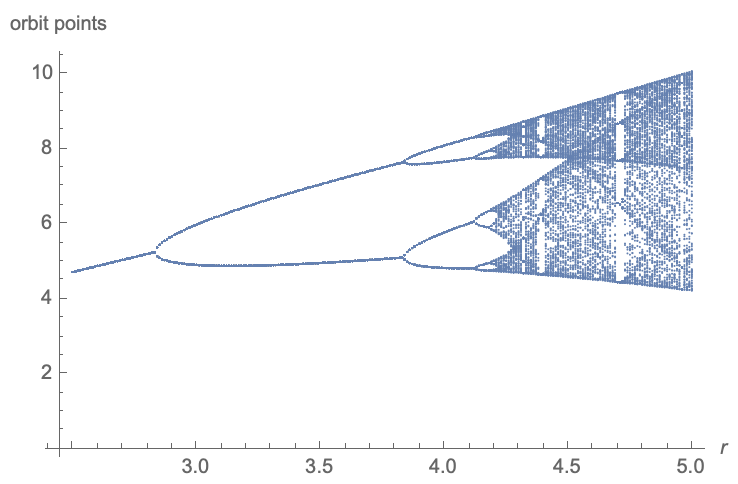
\includegraphics[scale=0.8]{img/191108-C27p5b.png}

What is it similar to?  Can you find a period-6 window? 

\emph{It looks like I didn't go to large enough $c$ for the obvious period-3 window to show up.}

\part Here are some trajectories of the Rossler system at various values of $c$.  You can hopefully see the periodic structures from the orbit diagram manifest as trajectories in phase space.

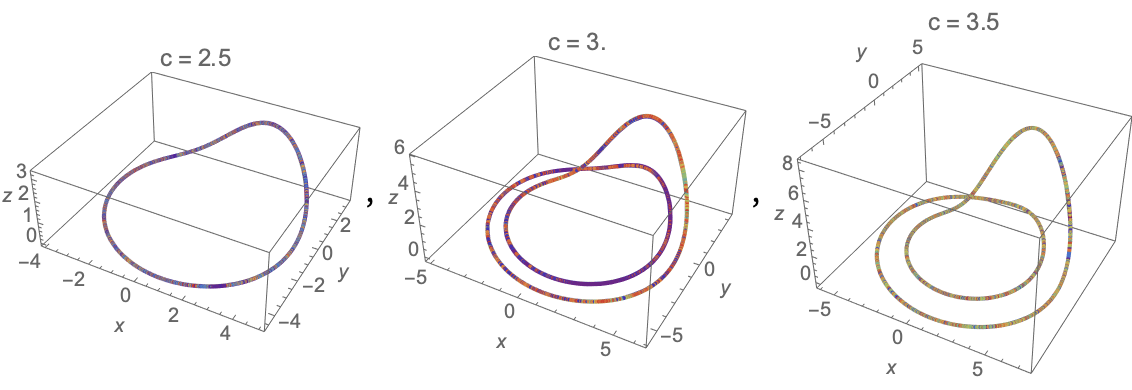
\includegraphics[width=0.7\textwidth]{img/191108-C27p5e.png}

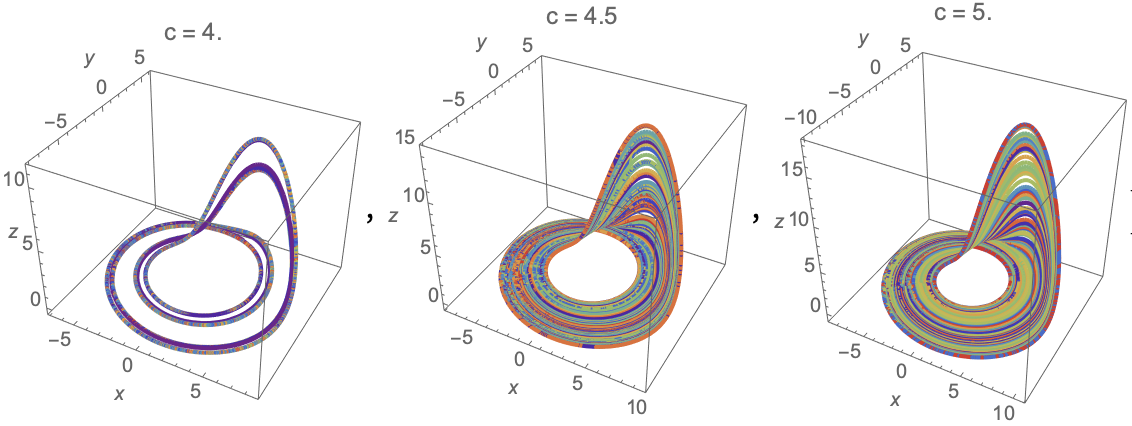
\includegraphics[width=0.7\textwidth]{img/191108-C27p5f.png}

What are the periods you see?  Which ones seem aperiodic?

\end{parts}
\end{questions}

1a: 10: $k/9$ for $k=0,1,2...0$.  Note that $0.999... = 9/9 = 1.$.  The slope is $10$ at each of them, so unstable.
1b: $0.10101010...$ would be period-2.
1c: $0.101001000100001...$ would be aperiodic.  So would $pi -3$ or $\sqrt{2} = 1$ as those have non-repeating decimal expansions.  Any irrational number, in fact!  So almost all points in the interval $[0,1]$ will have an aperiodic orbit.

1d: Decimal shift map: nearby points are pulled apart by a factor of $10$ by the map ('stretching').  In addition, nearby points like $0.10$ and $0.11$ can map far apart under the action of this map (to $0.0$ and $0.1$), so we call the map `tearing'

With the logistic map, for $r$ large enough, the interval $[0,1]$ is also stretched: nearby fixed points because further apart , meaning that the arc of $f(x)$ is longer than $1$ unit.  However, that map sort of bends (no discontinuities), so nearby points do always map to near each other.


2a: It looks like a tent (stretching factor of 3).

2b: Fixed points are $0$ and $3(1-x) = x$ so $3-3x = x$ so $x = 3/4$.

Mapping to zero: $0$ and $1$ map to zero.

Mapping to $0$ or $1$: $1/3$ maps to $1$ and so does $2/3$.

Mapping to $0$, $1$, $1/3$, $2/3$: $1/9$ and $2/9$ map to $1/3$ and $2/3$.  In addition, $7/9$ and $8/9$ do too.

2c: the stuff that leaves is the stuff that maps to above $1$.  $f(1/3) = 1$ and $f(2/3) = 1$.  For $1/3 < x < 2/3$, $f(x)>f(1/3)$, so that is the range that leaves.  The sketch is two lines.

2d: $[0,1/9], [2/9,1/3], [2/3,7/9], [8/9,1]$ stay in, so those four segments should be the sketch.
2e: Each segment in $C_2$ gets two little segments in $C_3$.  That will keep happening so lots of little segments in $C_k$.
2f: The limit of this process: hard to describe!

3a: period-1, period-2, period-4.
3b: flip bifurcation / period-doubling bifurcation.

4a: There's one.  It is the $xz$ in the third equation.

4b: This looks like the logistic orbit diagram.  There is a visible period-6 window between $4.3$ and $4.4$.

4c: $c=2.5$: period-1.  $c = 3$: period-2.  $c=3.5$: period 2.  $c = 4$: I am seeing four, I think, so period 4 (and I confirmed that by looking at the orbit diagram).  $c= 4.5$ and $c=5$: look aperiodic.


\end{document}